\section{Introduction}\label{sec:intro}

Maestro is a framework built for orchestrating co-simulations based on the
Functional Mock-Up Interface 2.0 standard for co-simulation.

The framework is divided into two parts: Maestro-Program and Maestro-Runtime.
\begin{description}
  \item[Maestro-Program] concerns the specification of a co-simulation. Such a
    specification is referred to as Maestro-ProgramSpecification, or
    ProgramSpecification when the context is clear. A ProgramSpecification consists
    of commands to be carried out by the Maestro-Runtime. In order to create a
    ProgramSpecification, Maestro-Program employs plugins that each provides
    fragments of the ProgramSpecification, which Maestro-Program then merges.
  \item[Maestro-Runtime] concerns the execution of a ProgramSpecification.

\end{description}

The flow of conducting a co-simulation using Maestro is depicted in
\cref{fig:conducting_co-simulation-overview}. The following paragraphs describes
the content of the figure. Initially, some terminology and definitions are
presented followed by a description of the consecutive behavior.
\begin{description}
  \item[Environment] An environment is data and information related to the
    co-simulation. For example, the FMUs to employ in a given co-simulation or the dependencies between the variables of the FMUs for a
    given co-simulation.
    \item[Program Environment] Terminology for Environment being used in context
    of Maestro-Program. The terminology only applies to naming for descriptive purposes.
    \item[Runtime Environment] Terminology for Environment being used in context
    of Maestro-Runtime. For example, a Program Environment passed to
    Maestro-Runtime becomes a Runtime Environment. The terminology only applies to naming for descriptive purposes.
    \item[Root Environment] Terminology for the initial Program Environment. The
    Root Environment typically consists of the FMUs to use in a co-simulation and values for FMU
    parameters. The terminology only applies to naming for descriptive purposes.
    \item[ProgramSpecification] A ProgramSpecification is a complete
    specification of a co-simulation to be carried out. A non-complete
    specification is referred to as a ProgramSpecification Fragment.
  \item[ProgramSpecification Fragment] A ProgramSpecification Fragment is part
    of a ProgramSpecification.
  \item[Plugin] A plugin can create a ProgramSpecification Fragment and/or add
    information to the environment. An example of environment information that a
    plugin can add is the dependencies between the variables of the FMUs. An example
    of a ProgramSpecification Fragment that a plugin can create is the necessary
    commands to perform initialisation of the FMUs.
\end{description}

The Activator in \cref{fig:conducting_co-simulation-overview} is the entity
(person or tool) that launches a co-simulation. The Activator shall provide a
Root Environment, see TODO, and a configuration of the plugins, see TODO.

Maestro-Program invokes the plugins according to the plugin configuration. This
is demonstrated in \cref{fig:conducting_co-simulation-overview} where Plugin 1
receives the Root Environment, and creates a new Environment, Environment 1, and
ProgramSpecification Fragment 1. This new environment is passed to Plugin 2,
which creates Environment 2 and ProgramSpecification Fragment 2. Finally, Plugin
N represents that this process can continue for several plugins.
At the end of this process, Maestro-Program will have assembled a
ProgramSpecification based on the ProgramSpecification Fragments created by the
plugins.

Maestro-Runtime executes the ProgramSpecification and can utilise the Runtime
Environment. In cases where Maestro-Runtime require
additional information on how to continue, it will query a
given plugin for such information. An example of such a case is debugging.


\begin{figure}[htb] \centering
  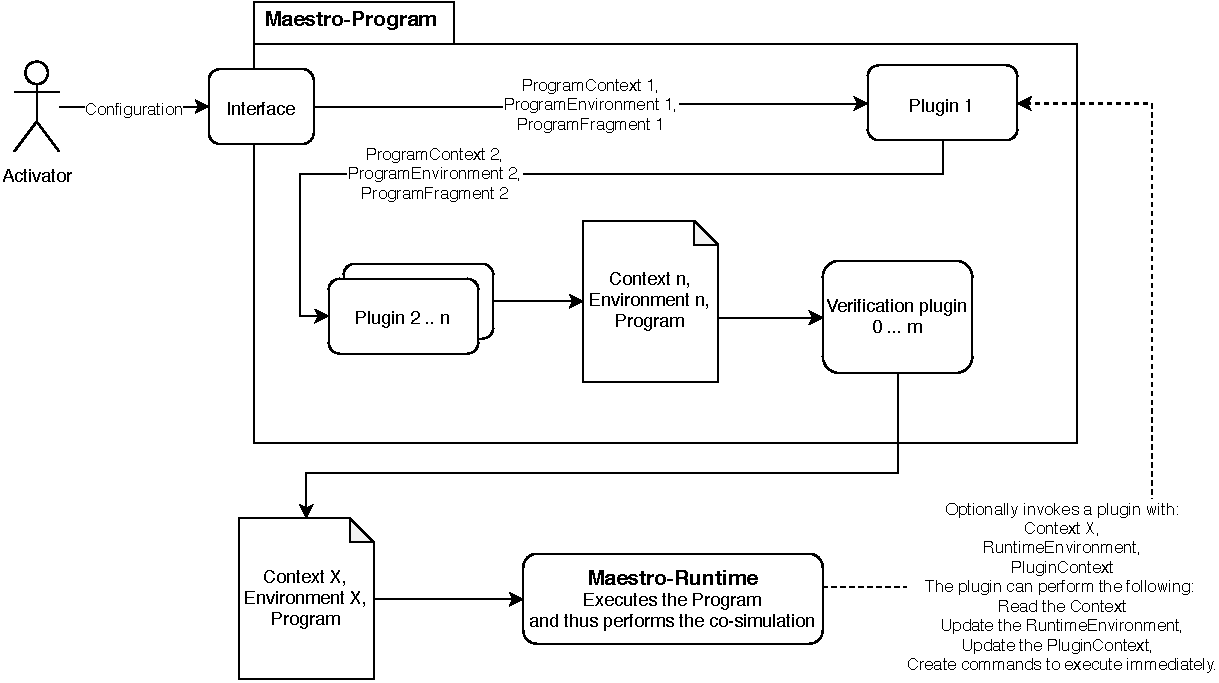
\includegraphics[width=\textwidth]{figures/conducting_co-simulation_overview.pdf}
  \caption{Conducting a co-simulation with Maestro-Program and Maestro-Runtime}
  \label{fig:conducting_co-simulation-overview}
\end{figure}

\subsection{TO BE DONE}
\begin{itemize}
  \item Validation of ProgramSpecification
  \end{itemize}

%%% Local Variables: %%% mode: latex %%% TeX-master: "../Maestro" %%% End:
